\documentclass[12pt,a4paper,titlepage]{article}

\usepackage{preamble}
\title{Représentation  Temps-Fréquence : travaux pratiques}
\author{Saâd Alaoui, Yassine Jamoud, Samy Haffoudhi}
\date{\today}

\begin{document}

\maketitle

\section{Présentation du TP}

Ce TP concerne l'imagerie Synthetic Apperture Focusing Technique (SAFT) pour le
contrôle par ultrasons. Nous nous intéressons au contrôle d'un bloc d'aluminium
contenant des petits trous à l'aide d'une sonde multi-élément en contact direct
avec la pièce. Nous mettrons en œuvre une méthode d'imagerie dite temporelle que
nous commencerons par implémenter dans matlab à l'aide de boucles \texttt{for} avant
de convertir ce code en fonction MEX afin de comparer le temps de calcul des deux
mises en œuvre.

\begin{figure}[H]
    \caption{Principe de l'imagerie SAFT}
    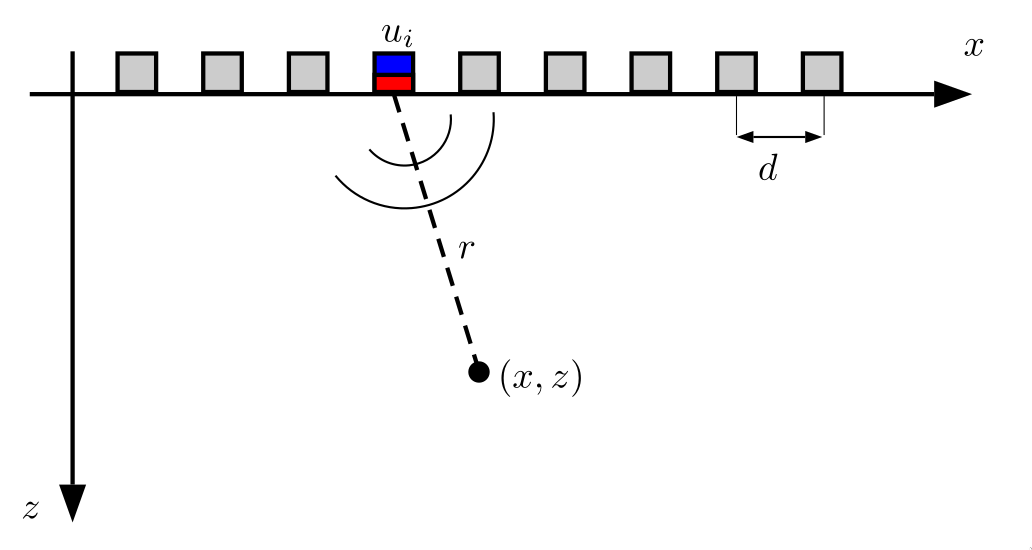
\includegraphics[width=0.6\textwidth]{sujet}
    \centering
\end{figure}

\section{Ouverture du fichier}

\begin{itemize}
    \item{On a $N_t = 1500$ et $N_{el} = 128$.}
    \item{Affichons l'image des données en fonction de $t$ et $u$ :

            \begin{figure}[H]
                \caption{Image des données}
                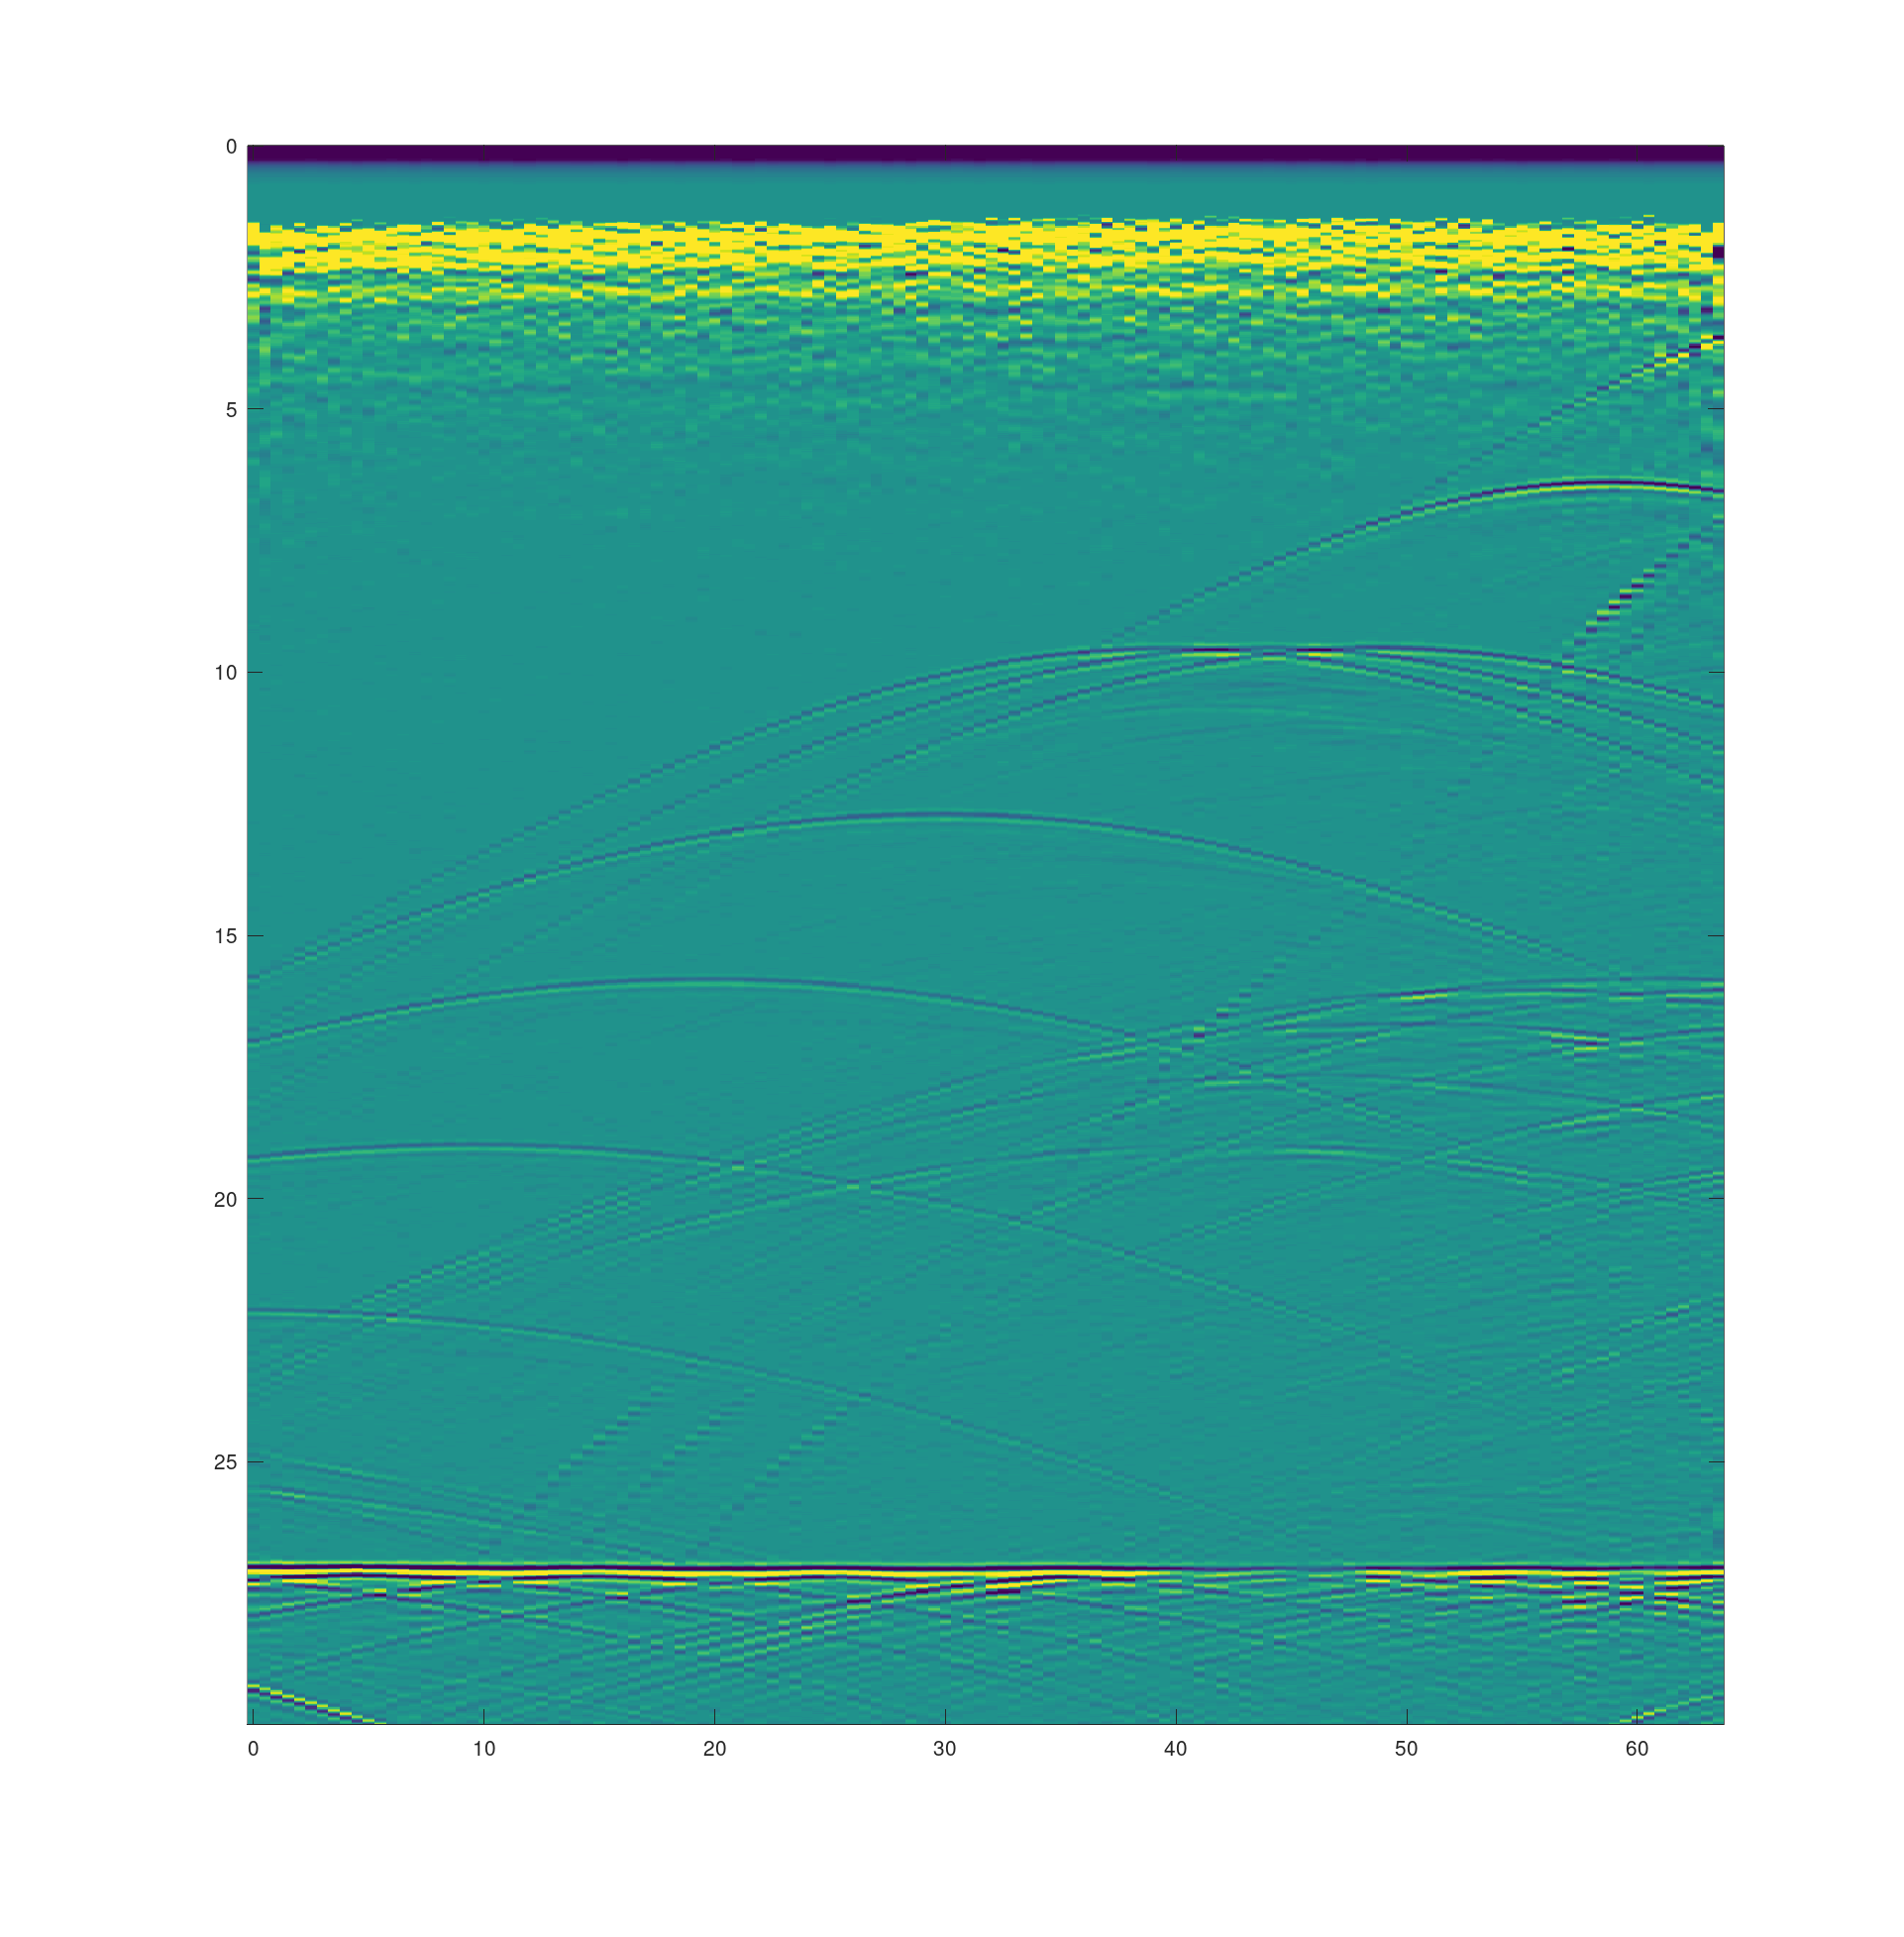
\includegraphics[width=0.5\textwidth]{im1}
                \centering
            \end{figure}
        }
    \item{Cette image n'est pas exploitable, on est incapable d'y distinguer les
        petits trous du bloc d'aluminium.}
    \item{Affichons maintenant un Ascan :

            \begin{figure}[H]
                \caption{Ascan}
                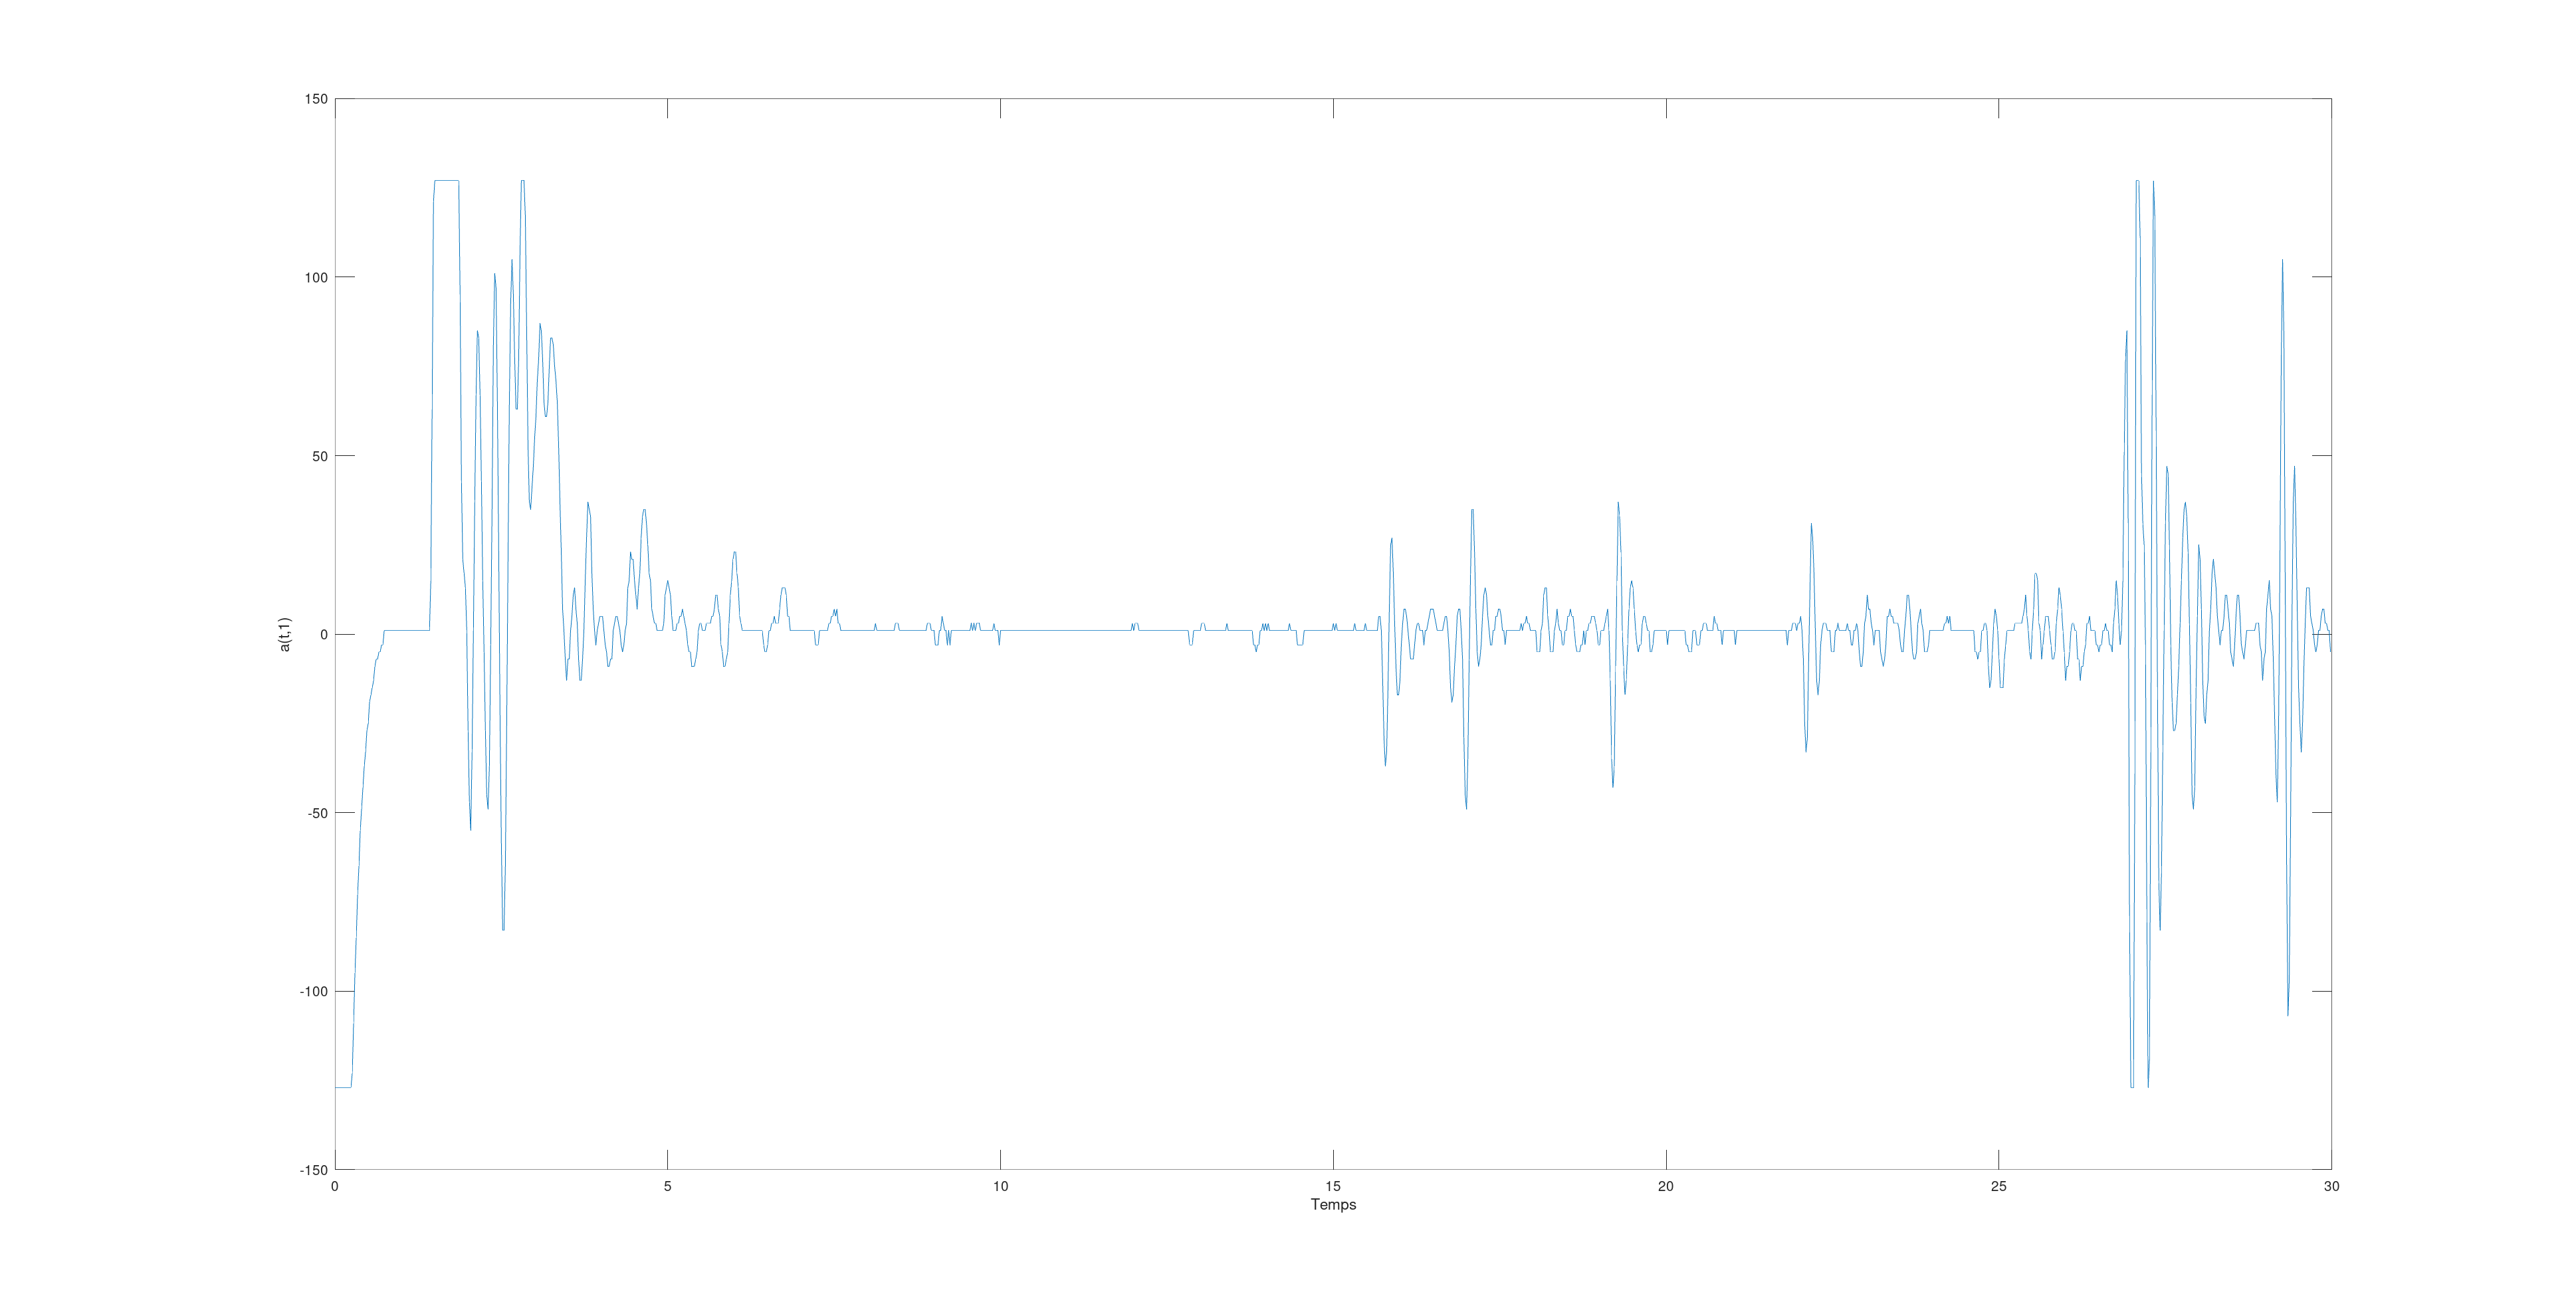
\includegraphics[width=0.7\textwidth]{im2}
                \centering
            \end{figure}
        }
    \item{On déduit de la figure précédente que $log_2(2 \times 128) = 8$ bits sont utilisés.}
\end{itemize}

\section{Définition de la grille de reconstruction}

Nous modifions le fichier \texttt{main.m} disponible en annexe.

\section{Reconstruction de l'image par une méthode temporelle}

\begin{itemize}
    \item{D'après la figure 2, on a : $r(x,z,u_i) = \sqrt{(u_i - x)^2 + z^2}$.}
    \item{On a : $\tau(x, z, u_i) = \frac{2r(x,z,u_i)}{c}$.}
    \item{Donc, on peut calculer $O(x,z) = \sum_{i=1}^{N_{el}}a(\tau(x, z, u_i),i)$.}
    \item{On ajoute la procédure au fichier \texttt{main.m} pour le calcul de $O$.}
    \item{Affichons l'image obtenue pour $N_x \in \{64,128,256,512,1024,2048\}$:
        }
\end{itemize}

\end{document}
